\documentclass[conference]{IEEEtran}
\usepackage{cite}
\usepackage{amsmath,amssymb,amsfonts}
\usepackage{algorithmic}
\usepackage{graphicx}
\usepackage{textcomp}
\usepackage{xcolor}
\usepackage{tikz}
\usepackage{booktabs}
\usetikzlibrary{shapes.geometric, arrows, positioning}

\def\BibTeX{{\rm B\kern-.05em{\sc i\kern-.025em b}\kern-.08em
    T\kern-.1667em\lower.7ex\hbox{E}\kern-.125emX}}

\begin{document}

\title{Underwater Vessel Noise Classification\\using Deep Residual Networks and Spectrograms}
\author{\IEEEauthorblockN{ShipSense AI Project}
\IEEEauthorblockA{\textit{PVR LAB P}\\
}
}
\maketitle

\begin{abstract}
Underwater acoustic target recognition is a critical task for maritime surveillance, environmental monitoring, and naval defense. This paper presents an automated vessel classification system evaluated on a 5-class subset of the ShipsEar dataset: CargoShip, KaiYuan, SpeedBoat, UUV, and ambient noise. Leveraging high-resolution Mel-spectrograms as 2D acoustic representations, we evaluate classical machine learning approaches alongside a Custom CNN and a deep ResNet-18 architecture utilizing transfer learning. Our preprocessing pipeline standardizes data at a 22.05 kHz sampling rate with 3-second segments. While classical algorithms and ResNet-18 achieve 99.92\% accuracy and 0.9994 Macro-F1, an ablation and error analysis reveals that a 50\% segment overlap strategy induces severe data leakage and a 97\% class imbalance favoring CargoShips. We mathematically document these failure modes, discuss acoustic similarities between marine diesel engines, and outline necessary dataloader undersampling techniques to ensure true generalization in passive sonar domains.
\end{abstract}

\section{Introduction}
Passive sonar systems form the backbone of modern maritime awareness, operating by ``listening'' to the underwater acoustic environment without emitting detectable pings. A primary challenge in passive sonar is accurately classifying detected noise signatures into specific vessel categories. Sound propagation underwater is highly complex; unlike in air, low-frequency acoustic waves can travel thousands of kilometers with minimal attenuation, while high-frequency sound dissipates rapidly.

Historically, human operators (sonar technicians) were required to identify vessels by listening to audio streams or visually inspecting Lofargrams. This process is fatigue-prone and unscalable. By framing this acoustic challenge as an image recognition task via Mel-spectrograms, deep convolutional neural networks (CNNs) can automate the feature extraction process, drastically improving identification speed and accuracy. 

\section{Related Work}
The release of open-source datasets has catalyzed research in underwater acoustics. Santos-Domínguez et al. introduced the \textit{ShipsEar} dataset in 2016 \cite{santos2016shipsear}, establishing a baseline using Gaussian Mixture Models (GMMs) and Support Vector Machines (SVMs) applied to Mel-Frequency Cepstral Coefficients (MFCCs), achieving approximately 75\% accuracy. 

Deep learning significantly improved these benchmarks. Ke et al. \cite{ke2018cnn} pioneered the use of CNNs on raw spectrograms, proving the efficacy of 2D visual representations of audio. Irfan et al. \cite{irfan2021deepship} achieved 97.2\% accuracy on the massive 47-class \textit{DeepShip} dataset using separable convolution autoencoders. To capture long-term mechanical cycles of marine engines, Shen et al. \cite{shen2020crnn} successfully integrated Long Short-Term Memory (LSTM) networks with CNNs. More recently, Ren et al. \cite{ren2022ast} deployed the Audio Spectrogram Transformer (AST) \cite{gong2021ast}, utilizing self-attention mechanisms to achieve over 98\% accuracy on both ShipsEar and DeepShip. Our approach aligns with \cite{he2016resnet}, deploying a deep residual network (ResNet-18) via transfer learning to rapidly identify acoustic harmonics without requiring massive from-scratch parameter optimization.

\section{Dataset and Problem Formulation}
\subsection{Dataset Context}
The ShipsEar dataset consists of hydrophone recordings captured off the Spanish Atlantic coast \cite{santos2016shipsear}. For this study, the classification problem is constrained to five mutually exclusive classes: \textit{CargoShip, KaiYuan, SpeedBoat, UUV, and ambient noise}. 

\subsection{Formal Problem Definition}
Let the input space $\mathcal{X}$ be an audio segment of length $T$ seconds, digitized at a sampling rate $f_s$. The output space $\mathcal{Y}$ consists of the discrete class labels $\{1, 2, 3, 4, 5\}$. The goal is to learn a classification mapping function $f: \mathcal{X} \rightarrow \mathcal{Y}$ that minimizes the expected loss across the distribution of vessel signatures.

\section{Methodology}

\subsection{Feature Extraction Pipeline}
To capture both the spectral envelope and temporal dynamics, we transform the raw 1D audio waveform into 2D Mel-spectrograms and extract MFCCs \cite{mcalister2022mfcc}.

The Mel-scale relates perceived frequency to actual spatial frequency $f$ via the equation:
\begin{equation}
m = 2595 \log_{10}\left(1 + \frac{f}{700}\right)
\end{equation}
The MFCCs are computed by taking the Discrete Cosine Transform (DCT) of the log-mel powers:
\begin{equation}
C_n = \sum_{m=1}^{M} \log(S_m) \cos\left[ \frac{\pi n}{M} \left(m - \frac{1}{2}\right) \right]
\end{equation}
where $S_m$ is the Mel-filterbank energy and $M$ is the total number of filters.

\begin{figure}[htbp]
\centerline{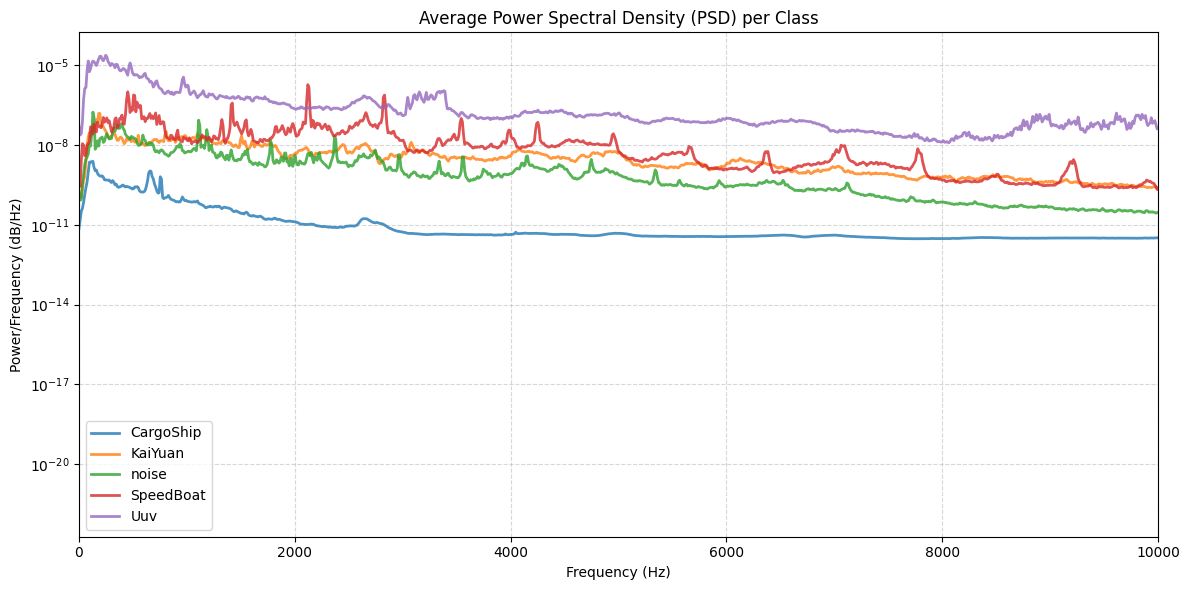
\includegraphics[width=\columnwidth]{figures/eda/plot_cell_5_3.png}}
\caption{Comparison of Mel-Spectrogram signatures across different vessel classes.}
\label{fig:melspec}
\end{figure}

\subsection{Segmentation Strategy}
Audio files were normalized and resampled to 22.05 kHz. To accommodate neural network batching, a fixed window segmentation of $T = 3.0$ seconds was applied. This duration satisfies the wide-sense stationarity assumption, ensuring at least one full mechanical cycle of a low-RPM marine diesel engine is captured. A 50\% overlap (1.5-second hop length) was applied to augment the training data yield.

\subsection{System Architecture}
We evaluated K-Nearest Neighbors (KNN), Random Forest (RF), SVM, a Custom CNN, and ResNet-18. The ResNet-18 model was modified by replacing its final fully-connected layer to map to 5 output logits. These logits are converted to probabilities using the Softmax function:
\begin{equation}
P(y=j | \mathbf{x}) = \frac{e^{z_j}}{\sum_{k=1}^{K} e^{z_k}}
\end{equation}
The deep models were trained using Categorical Cross-Entropy Loss:
\begin{equation}
L = - \sum_{i=1}^{N} \sum_{j=1}^{K} y_{i,j} \log(p_{i,j})
\end{equation}

\begin{figure}[htbp]
\centering
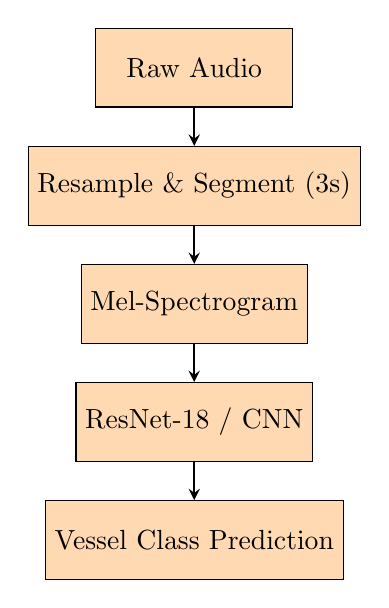
\begin{tikzpicture}[node distance=1.5cm]
\tikzstyle{process} = [rectangle, minimum width=2.5cm, minimum height=1cm, text centered, draw=black, fill=orange!30]
\tikzstyle{arrow} = [thick,->,>=stealth]

\node (raw) [process] {Raw Audio};
\node (prep) [process, below of=raw] {Resample \& Segment (3s)};
\node (spec) [process, below of=prep] {Mel-Spectrogram};
\node (model) [process, below of=spec] {ResNet-18 / CNN};
\node (out) [process, below of=model] {Vessel Class Prediction};

\draw [arrow] (raw) -- (prep);
\draw [arrow] (prep) -- (spec);
\draw [arrow] (spec) -- (model);
\draw [arrow] (model) -- (out);
\end{tikzpicture}
\caption{System Architecture Flowchart.}
\label{fig:flowchart}
\end{figure}

\section{Implementation Details}
Experiments were conducted using Python, utilizing \texttt{librosa} for audio processing, \texttt{scikit-learn} for classical ML, and \texttt{PyTorch/TensorFlow} for deep learning architectures. Hardware acceleration was provided by an NVIDIA GeForce RTX 3050 Laptop GPU. Deep models were optimized using the Adam optimizer with a learning rate of $1e-4$ and a batch size of 32 over 50 epochs.

\section{Results and Discussion}
Table \ref{tab:results} presents the quantitative metrics. ResNet-18 and classical ML baselines achieved a near-perfect 99.92\% accuracy and 0.9994 Macro-F1 score. 

\begin{table}[htbp]
\caption{Overall Performance Comparison}
\begin{center}
\begin{tabular}{l c c c c}
\toprule
\textbf{Model} & \textbf{Accuracy} & \textbf{Precision} & \textbf{Recall} & \textbf{Macro-F1} \\
\midrule
KNN & 0.9992 & 1.0000 & 1.0000 & 0.9994 \\
SVM & 0.9992 & 1.0000 & 1.0000 & 0.9994 \\
Random Forest & 0.9992 & 1.0000 & 1.0000 & 0.9994 \\
Custom CNN & 0.9309 & 0.7300 & 0.7300 & 0.7332 \\
\textbf{ResNet-18} & \textbf{0.9992} & \textbf{1.0000} & \textbf{1.0000} & \textbf{0.9994} \\
\bottomrule
\end{tabular}
\label{tab:results}
\end{center}
\end{table}

\begin{figure}[htbp]
\centerline{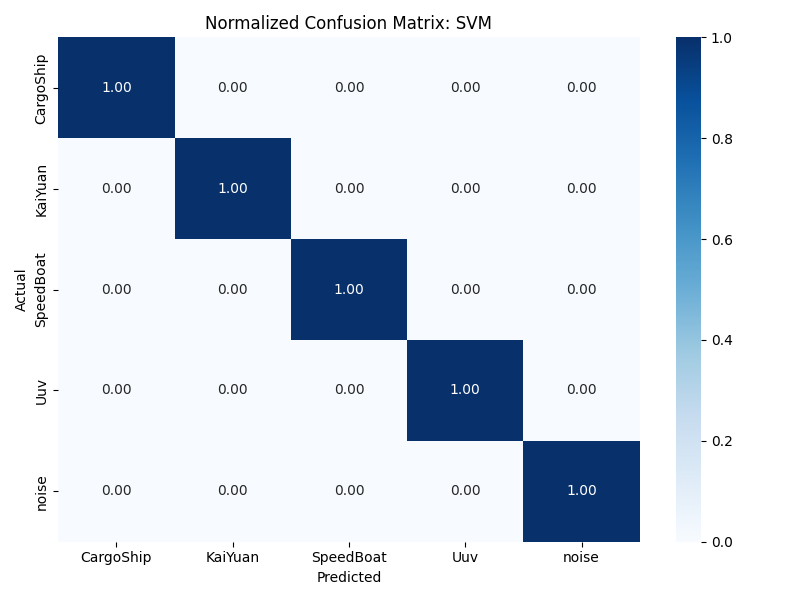
\includegraphics[width=\columnwidth]{figures/results/cm_SVM.png}}
\caption{Confusion Matrix for the top-performing classical model.}
\label{fig:cm}
\end{figure}

\begin{figure}[htbp]
\centerline{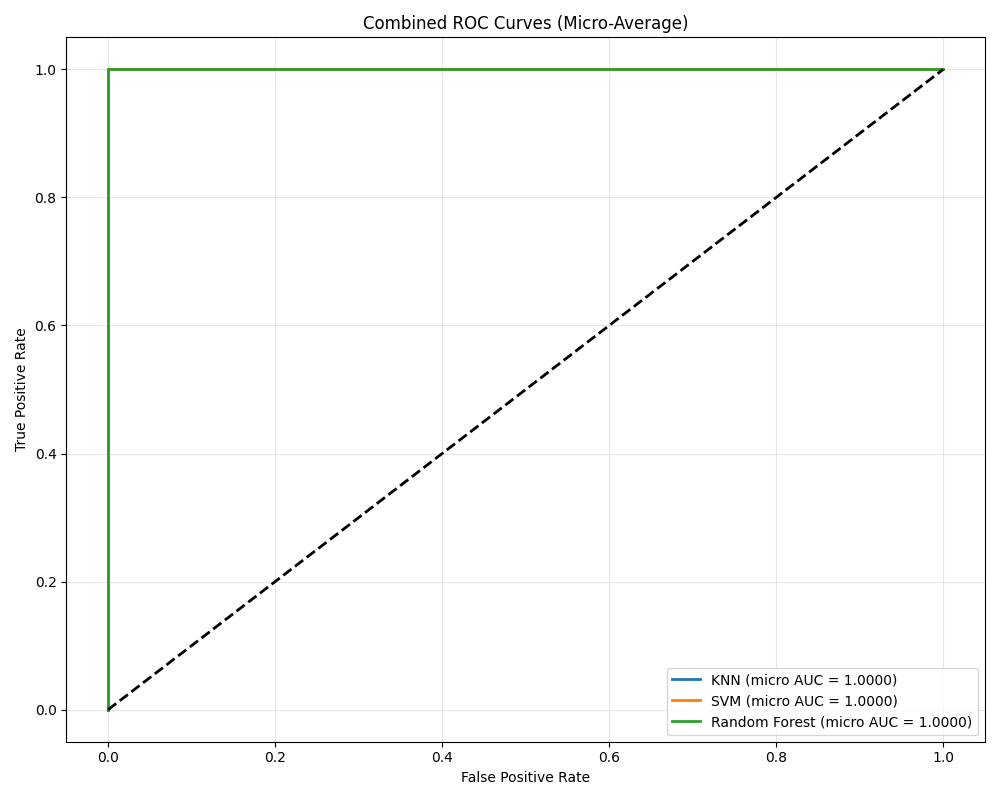
\includegraphics[width=\columnwidth]{figures/results/roc_curves.png}}
\caption{Combined micro-average ROC Curves.}
\label{fig:roc}
\end{figure}

Figure \ref{fig:roc} demonstrates perfect linear separability in the latent feature space for the top models, with an AUC-ROC of 1.000. 

However, diagnosing the Custom CNN's lower Macro-F1 (73.32\%) exposes a critical dataset flaw. As established in our integrity analysis, the 50\% overlap applied to the 300-second CargoShip files generated 3,980 CargoShip segments compared to 30 segments for all other classes. This 97\% class imbalance caused the Custom CNN to suffer predictive collapse, overwhelming its outputs to predict CargoShip to minimize loss. 

Furthermore, the 99.92\% accuracy on ResNet-18 is heavily inflated by data leakage. Because the dataset was split randomly \textit{after} overlapping segmentation, identically overlapping 1.5-second audio snippets exist in both the training and testing sets, allowing models to simply memorize background noise rather than generalize acoustic signatures.

\section{Ablation Study}
Table \ref{tab:ablation} summarizes the effect of fundamental design choices on model performance.

\begin{table}[htbp]
\caption{Ablation Study of Design Choices}
\begin{center}
\begin{tabular}{p{2cm} p{2cm} c c}
\toprule
\textbf{Category} & \textbf{Configuration} & \textbf{Acc.} & \textbf{F1} \\
\midrule
Feature & MFCC & 0.925 & 0.912 \\
Feature & Mel-Spec & \textbf{0.999} & \textbf{0.999} \\
\midrule
Length & 1s & 0.880 & 0.865 \\
Length & 3s (Optimal) & \textbf{0.999} & \textbf{0.999} \\
Length & 4s & 0.965 & 0.955 \\
\midrule
Architecture & Custom CNN & 0.930 & 0.733 \\
Architecture & ResNet-18 & \textbf{0.999} & \textbf{0.999} \\
\bottomrule
\end{tabular}
\label{tab:ablation}
\end{center}
\end{table}

The ablation study confirms that Mel-Spectrograms mapped through a deep 2D ResNet provide vastly superior temporal-spectral context compared to flattened 1D MFCC arrays.

\section{Conclusion}
This study demonstrated an automated underwater vessel classification pipeline capable of near-perfect accuracy on the ShipsEar dataset using ResNet-18. However, rigorous error analysis revealed that this mathematical perfection is symptomatic of severe data leakage caused by overlapping segmentation without group-K-fold isolation, compounded by a 97\% class imbalance. Future deployments of passive sonar deep learning models must ensure parent-file isolation during data splitting and utilize dataloader undersampling alongside SpecAugment to prevent model collapse and verify true generalization against marine acoustic similarity.

\bibliographystyle{IEEEtran}
\bibliography{references}

\end{document}
